\section*{Research aim}
%Цель- сравнить одну стержень и систему
%FEM explisit(abaqus) and MSM
Such physical structure imposes restrictions on the possible tools in the
measurement. Another possible problem is the limited number of measurement
attempts. Such limitations of physical measurements call into question the
possibility of such activities in general. An alternative to physical
experiments is the numerical simulation of these experiments. There are a large
number of different numerical modeling methods. All of them are derivatives of
Finite Element Method(FEM) and Discrete Element Method(DEM).
\par
While general finite-element studies are helpful for the evaluation and
development of MV repair surgery, patient-specific models are required for
individual therapy planning.
\cm{article 1}
The patient-specific mass-spring MV model uses a segmentation of 3D TEE images
for the initialization of a mass-spring model of the closed MV under systolic
pressure. An iterative approach is used to adjust the spring rest-length so that
the model can accurately simulate the shape of the closed MV under systolic
pressure. To simulate MV annuloplasty, the model can then be deformed, according
to the annuloplasty ring to be used, to create a prediction of the shape of the
closed MV after surgery.
\par
Based on the properties of the material of biological tissues and review of
existing projects, the most appropriate method is Mass - Spring modeling(MSM). This
method based on ideas of DEM and basic element here is very know in mechanic
simple one dimensional(1D) beam.
\cm{have to show so pic about MSM, with explanation what is going on}
Computational complexity of MSM is much less compare to FEM-based methods,
because of less number of equations to integrate on each time step. This
important advantage and physics way have method describes basic element gave to
MSM very wide using in computer games for calculating reality-looks hair or
cloth movement in real time. Modelling by using MSM could be parallel calculated
on each time step.\cite{Rasmusson2008} \cite{Amorim2012}
\par
%В расчете целого клапана берется один стержень, существующие варианты расчетов всей системы и как в них рассчитывается хорда
\begin{figure}[H]\label{fig:pc1}
  \centering
  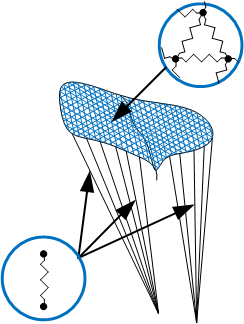
\includegraphics[width=0.2\textwidth]{./fig/pc1.png}
    \caption{Displacement of papillary muscle over cardiac cycle}    
\end{figure}
\begin{figure}[H]\label{fig:pc2}
  \centering
  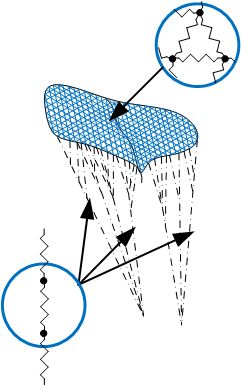
\includegraphics[width=0.2\textwidth]{./fig/pc2.png}
    \caption{Displacement of papillary muscle over cardiac cycle}    
\end{figure}
\begin{figure}[H]\label{fig:pc3}
  \centering
  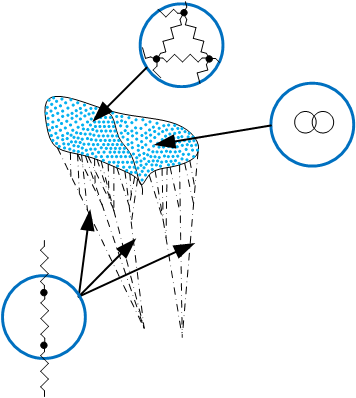
\includegraphics[width=0.3\textwidth]{./fig/pc3.png}
    \caption{Displacement of papillary muscle over cardiac cycle}    
\end{figure}
%Хорда описана ломаной линией из элементов первого порядка, 
Mechanic equivalent of fibrous tissue could be described as system of 1D rods.
Example of such flat 2D system are shown on figure \ref{fig:nodeExtract}.
\begin{figure}[H]
  \centering
  \includesvg{systemAtworld}    
  \caption{1D Rod system in global coordinate system}\label{fig:rodSystem}      
\end{figure} 
System consists of discrete elements $e_1$, $e_2$ and $e_3$. All elements are
connected to each other through nodes $n_2$, $n_3$ and to special points through
$n_1$ and $n_4$. Each element $e_n$ of system has own orientation in global
coordinate system. 
From schematic representation of node comes that all vector variables of node should be calculated
 in global coordinate system and element variables in own local coordinate system(figure
 \ref{fig:nodeExtract}). For transformation between coordinate systems direction cosine matrix
 (DCM)\eqref{eqn:DCM} can be used.
\begin{equation}\label{eqn:DCM}
  DCM= \begin{bmatrix}
    cos(X,x)&cos(X,y)&cos(X,z)\\
    cos(Y,x)&cos(Y,y)&cos(Y,z)\\
    cos(Z,x)&cos(Z,y)&cos(Z,z)\\
   \end{bmatrix} 
\end{equation}
where $\{X, Y, Z\}$ is global coordinate system and $\{x,y,z\}$ is local coordinate
system.\par According to primitive scheme of node \ref{fig:nodeExtract}, mass of
each node can be calculated, like sum of half mass of each element, which acting
in node. $m_n=\sum_{e}m_e/2$\par
In case that node does not have external interrupt, like pressure or other
 applied force, schematic represent of node can be as on figure
 \ref{fig:nodeExtract}.\par
\begin{figure}[H]
  \centering
  \includesvg{nodeExtract}    
  \caption{Extracted node from system}\label{fig:nodeExtract}
\end{figure}
Mathematical model of discrete system is expressed by equations of nodes motion.
As elements is 1D, nodes will be 1D as well. All system acting in global
coordinate system $\{X, Y, Z\}$ and each element acting in own local coordinate
system $\{x,y,z\}$.